\documentclass{article}
\usepackage{fancyhdr}
\usepackage{extramarks}
\usepackage{amsmath}
\usepackage{amsthm}
\usepackage{amsfonts}
\usepackage{enumitem}
\usepackage{graphicx}
\usepackage[cspex,bbgreekl]{mathbbol}

\topmargin=-0.45in
\evensidemargin=0in
\oddsidemargin=0in
\textwidth=6.5in
\textheight=9.0in
\headsep=0.25in
\pagestyle{empty}
\linespread{1.5}

\def \grad{\nabla}
\def \p{\partial}

\def \CC{\mathbb{C}}
\def \FF{\mathbb{F}}
\def \II{\mathbb{I}}
\def \RR{\mathbb{R}}
\def \PP{\mathbb{P}}
\def \SS{\mathbb{S}}
\def \EE{\mathbb{E}}
\def \KK{\mathbb{K}}
\def \bs{\boldsymbol}
\def \mc{\mathcal}

\renewcommand\headrulewidth{0.4pt}
\renewcommand\footrulewidth{0.4pt}

\setlength\parindent{0pt} % Removes all indentation from paragraphs


\begin{document}
From \textbf{5.5.4} The hydrostatic pressure is derived from the Cauchy stress tensor in the following way to decompose the Cauchy stress into a traceless deviatoric component and a diagonal dilational component. 
\[\bbsigma = \bbsigma' + p\II\]
\[p = \frac{1}{3}\text{tr}(\bbsigma)\]
The above can be stated in terms of PK1 using the standard transformation with the the resulting equalities.
\[\PP = \PP' + pJ\FF^{-T}\]
\[\PP':\FF = 0; p = \frac{1}{3}J^{-1}\PP:\FF\]

We we will generate the equation for an incompressible hyperelastic material from \textbf{6.5.1} in terms of PK1 for familiarity. The following statement is derived in \textbf{6.2}. 
\[\bigg(\PP - \frac{\p\Psi}{\p\FF}\bigg):\dot{\FF} = 0 \]
The following is a result of $J = 1$ for incompressible materials which implies $\dot J = 0$. This is a statement about the constraint on $\dot\FF$ given incompressibility.
\[\dot{J} = J\FF^{-T}:\dot{\FF} =  0\]
Combining the last two statements we end up with the following equation with an unknown scaling term $\gamma$.
\[\PP - \frac{\p\Psi}{\p\FF} = \gamma J\FF^{-T}\]
We can now state the general incompressible hyperelasic constitutive equation in terms of PK1.
\[\PP = \frac{\p\Psi}{\p\FF} + \gamma J\FF^{-T}\]
The factor $J$ is not removed from the above equality because $J = 1$ is not usually strictly enforced, and the above equation can be used for the nearly incompressible case. We can now try to find a relationship between $\gamma$ and the hydrostatic pressure, $p$.
\begin{align*}
    p &= \frac{1}{3}J^{-1}\PP:\FF \\
    &= \frac{1}{3}J^{-1}\frac{\p\Psi}{\p\FF}:\FF + \gamma
\end{align*}
This implies that for $\gamma = p$, we need to use the invariant form of the energy equations such that $\bar\Psi(\FF) = \Psi(\bar\FF)$, where $\bar\FF = J^{-1/3}\FF$. A proof is given on page 168, and covered more extensively in section \textbf{2.3.2} of Ben's paper.

We can use the previous results to model nearly incompressible materials, or help stabilize incompressible material solves by modifying the energy funcitonal, $\Psi$, to be the sum of $\bar\Psi$ and a volumetric penalty term $U(J)$. The penalty term needs to satisfy $U(1) = 0$ so now extra energy is introduced by this term when the volume is maintained. In the same vein we want $U(J)\to\infty$ as $J \to 0$ or $J\to\infty$ to penalize large contractions and dilations. For example, we commonly use $\frac{\kappa}{2}\log(J)^2$. PK1 can then be epressed in terms of the deviatoric and dilational components. 
\begin{align*}
    \PP &= \frac{\p\Psi}{\p\FF} \\
    &= \frac{\p\bar\Psi}{\p\FF} + \frac{dU}{dJ}\frac{\p J}{\p\FF} \\
    &= \frac{\p\bar\Psi}{\p\FF} + \frac{dU}{dJ}J\FF^{-T}
\end{align*}
This result implies that we can express $p$ in terms of the derivative of the energy penalty term.
\[p = \frac{dU}{dJ}\]
This equality places an additional constraint $U'(1) = 0$ so the dilational stress is 0 when the volume is maintained.
The major result of Ben's paper can be summed up in the following way. The most stable work conjugate formulas split the stress into dilational and deviatoric components, or $\Psi = \bar\Psi + U(J)$. I have included a summary figure for one of the benchmark tests he conducted.
\begin{figure}[ht]
\begin{center}
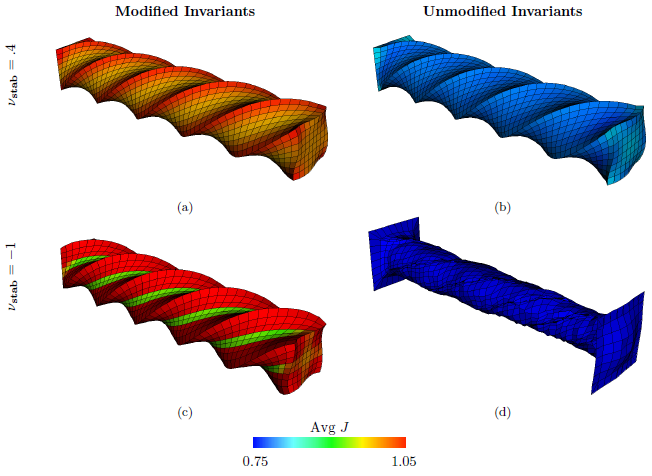
\includegraphics{twisting_beam.PNG}
\caption{Note that $\nu = -1$ implies no energy penalty term}
\end{center}
\end{figure}

I will now cover some changes in the methodology. The first change would be when the energy term cannot be expressed in terms of modified invariants, such as for Fung-type models. In that case you can use the deviatoric projection to find the deviatoric component of the stress, which, for PK1, can be computed in the following way.
\[\text{DEV}(\PP) = \PP - \frac{1}{3}(\PP:\FF)\FF^{-T}\]
For the most part we have been using PK1 within applications that have the dilational and deviatoric components combined when doing the force spreading. There is, however, a method that Simone thinks might reduce locking somewhat by splitting the terms within IBAMR so that different quadrature orders can be used fo each. For the pressure stabilization method, the pressure is computed using the derivative of $U$ and added to the final $\PP$ value independently of the deviatoric PK1 stress.
\[p = U'(J)\]
\[\PP_{p} = pJ\FF^{-T}\]
There are no concrete results on the efficacy of this method compared to the joint stress term with modified invariants and the penalty term.
\end{document}
